\documentclass[a4paper,oneside,12pt]{extreport}

\usepackage{mmap}
\usepackage[T2A]{fontenc}
\usepackage[utf8]{inputenc}
\usepackage[english,russian]{babel}

\usepackage[left=30mm, right=15mm, top=20mm, bottom=20mm]{geometry}

\setlength{\parindent}{1.25cm} % Абзацный отступ

\usepackage{setspace}
\onehalfspacing % Полуторный интервал

\frenchspacing % Равномерные пробелы
\usepackage{indentfirst} % Красная строка

\usepackage{microtype}
\sloppy

\usepackage{titlesec}
\titlespacing*{\chapter}{0pt}{-30pt}{8pt}
\titlespacing*{\section}{\parindent}{*4}{*4}
\titlespacing*{\subsection}{\parindent}{*4}{*4}
\titleformat{\chapter}{\LARGE\bfseries}{\thechapter}{20pt}{\LARGE\bfseries}
\titleformat{\section}{\Large\bfseries}{\thesection}{40pt}{\Large\bfseries}

\usepackage{graphicx}
\usepackage{caption}

\usepackage[unicode,pdftex]{hyperref}
\hypersetup{hidelinks}

\usepackage{amsmath}

%% title begin
\usepackage{wrapfig}

\makeatletter
	\def\vhrulefill#1{\leavevmode\leaders\hrule\@height#1\hfill \kern\z@}
\makeatother
%% title end

%% begin code
\usepackage{listings}
\usepackage{xcolor}

\lstset{
	basicstyle=\footnotesize\ttfamily,
	breakatwhitespace=true,
	breaklines=true,
	commentstyle=\color{gray},
	frame=single,
	keywordstyle=\color{blue},
	stringstyle=\color{red},
	tabsize=8
}

\newcommand{\code}[1]{\texttt{#1}}
%% end code


\begin{document}

\begin{titlepage}
	{\large % 14pt instead of 12pt
	\onehalfspacing
	\centering

	\begin{wrapfigure}[7]{l}{0.14\linewidth}
		\vspace{3mm}
		\hspace{-10mm}
		
\includegraphics[width=0.93\linewidth]{inc/img/bmstu-logo}
	\end{wrapfigure}
	{\singlespacing \footnotesize \bfseries Министерство науки и высшего образования Российской Федерации\\Федеральное государственное бюджетное образовательное учреждение\\высшего образования\\<<Московский государственный технический университет\\имени Н.~Э.~Баумана\\ (национальный исследовательский университет)>>\\(МГТУ им. Н.~Э.~Баумана)\\}

	\vspace{-2.2mm}
	\vhrulefill{0.9mm}\\
	\vspace{-7.5mm}
	\vhrulefill{0.2mm}\\
	\vspace{2mm}

	{\doublespacing \small \raggedright ФАКУЛЬТЕТ \hspace{37mm} «Информатика и системы управления»\\
	КАФЕДРА \hspace{17mm} «Программное обеспечение ЭВМ и информационные технологии»\\}

	\vspace{30mm}

	\textbf{ОТЧЁТ}\\
	По лабораторной работе № 2\\
	По курсу: «Моделирование»\\
	Тема: «Распределение случайных величин»\\
	Вариант: 6 $\equiv$ 2 (mod 4)\\

	\vspace{40mm}

	\begin{flushleft}
		\begin{tabular}{lr}
			\textbf{Студент:}        & Керимов~А.~Ш. \\
			\textbf{Группа:}         & ИУ7-74Б       \\
			\textbf{Оценка (баллы):} & \hrulefill    \\
			\textbf{Преподаватель:}  & Рудаков~И.~В. \\
		\end{tabular}
	\end{flushleft}

	\vfill

	Москва\\
	\the\year\\}
\end{titlepage}

\setcounter{page}{2}


\textbf{Цель работы.} Получение навыков разработки алгоритмов решения краевой задачи при реализации моделей, построенных на ОДУ второго порядка.

\section*{Исходные данные}

\begin{enumerate}
	\item Задана математическая модель.

	Уравнение для функции $T(x)$
	\begin{equation}
		\frac{\mathrm d}{\mathrm dx}\left(k(x)\frac{\mathrm dT}{\mathrm dx}\right)-\frac2R\alpha(x)T+\frac{2T_0}R\alpha(x)=0.
		\label{eqn:1}
	\end{equation}

	Краевые условия
	\begin{equation}
		\left\{
		\begin{aligned}
			x&=0,\quad-k(0)\frac{\mathrm dT}{\mathrm dx}=F0,\\
			x&=l,\quad-k(l)\frac{\mathrm dT}{\mathrm dx}=\alpha_N(T(l)-T_0).
		\end{aligned}
		\right.
	\end{equation}

	\item Функции $k(x)$, $\alpha(x)$ заданы своими константами
	\begin{equation}
		\begin{aligned}
			k(x)&=\frac a{x-b},\\
			\alpha(x)&=\frac c{x-d}.
		\end{aligned}
	\end{equation}
	Константы $a$, $b$ следует найти из условий $k(0)=k_0$, $k(l)=k_N$, а константы $c$, $d$ из условий $\alpha(0)=\alpha_0$, $\alpha(l)=\alpha(N)$.

	\item Разностная схема с разностным краевым условием при $x=0$.
	Получено в \href{ftp://eufs.bmstu.ru/19426610-bd1a-11e6-93f1-005056960017/26-03-2020-%D0%9B%D0%B5%D0%BA%D1%86%D0%B8%D1%8F_%E2%84%967_%D0%9C%D0%BE%D0%B4%D0%B5%D0%BB%D0%B8_%D0%9E%D0%94%D0%A3_%D0%BA%D1%80%D0%B0%D0%B5%D0%B2%D0%B0%D1%8F_%D0%B7%D0%B0%D0%B4%D0%B0%D1%87%D0%B0.pdf}{Лекции №7} (7.14), (7.15), и может быть использовано в данной работе.
	Самостоятельно надо получить интегро-интерполяционным методом разностный аналог краевого условия при $x=l$, точно так же, как это было сделано применительно к краевому условию при $x=0$ в Лекции №7 (7.15).
	Для этого надо проинтегрировать на отрезке $[x_{N-\frac12}, x_{N+\frac12}]$ выписанное выше уравнение \eqref{eqn:1} с учётом (7.9) из Лекции №7 и учесть, что поток $F_N=\alpha_N(y_N-T_0)$, а $\displaystyle F_{N-\frac12}=\chi_{N-\frac12}\frac{y_{N-1}-y_N}h$.

	\item Значения параметров для отладки (все размерности согласованы)
	\begin{equation*}
		\begin{array}{rlll}
			k_0      &=& 0,4  &\quad\text{Вт/см К},\\
			k_N      &=& 0,1  &\quad\text{Вт/см К},\\
			\alpha_0 &=& 0,05 &\quad\text{Вт/см² К},\\
			\alpha_N &=& 0,01 &\quad\text{Вт/см² К},\\
			l        &=& 10   &\quad\text{см},\\
			T_0      &=& 300  &\quad\text{К},\\
			R        &=& 0,5  &\quad\text{см},\\
			F_0      &=& 50   &\quad\text{Вт/см²}.\\
		\end{array}
	\end{equation*}
\end{enumerate}

\section*{Физическое содержание задачи}

Сформулированная математическая модель описывает температурное поле $T(x)$ вдоль цилиндрического стержня радиуса $R$ и длиной $l$, причём $R<<l$ и температуру можно принять постоянной по радиусу цилиндра.
Ось $x$ направлена вдоль оси цилиндра и начало координат совпадает с левым торчцем стержня.
Слева при $x=0$ цилиндр нагружается тепловым потоком $F_0$.
Стержень обдувается воздухом, температура которого равна $T_0$.
В результате происходит съем тепла с цилиндрической поверхности и поверхности правого торца при $x=l$.
Функции $k(x)$, $\alpha(x)$ являются, соответственно, коэффициентами теплопроводности материала стержня и теплоотдачи при обдуве.

\section*{Результаты работы}

\begin{enumerate}
	\item \textbf{Разностный аналог краевого условия при $x=l$ и его краткий вывод интегро-интерполяционным методом}

	Обозначим $\displaystyle F=-k(x)\frac{\mathrm dT}{\mathrm dx}$, $\displaystyle p(x)=\frac2R\alpha(x)$, $\displaystyle f(x)=\frac{2T_0}R\alpha(x)$.
	Тогда \eqref{eqn:1} примет вид:
	\begin{equation}
		-\frac{\mathrm dF}{\mathrm dx}-p(x)T+f(x)=0.
	\end{equation}

	Проинтегрируем на отрезке $[x_{N-\frac12}, x_{N+\frac12}]$:
	\begin{equation}
		-\int_{x_{N-\frac12}}^{x_N} \frac{\mathrm dF}{\mathrm dx}\,\mathrm dx
		-\int_{x_{N-\frac12}}^{x_N} p(x)T\,\mathrm dx
		+\int_{x_{N-\frac12}}^{x_N} f(x)\,\mathrm dx
		=0.
	\end{equation}

	Второй и третий интеграл вычислим методом трапеций:
	\begin{equation}
		F_{N-\frac12}-F_N
		-\frac{p_{N-\frac12}y_{N-\frac12}+p_Ny_N}2\cdot\frac h2
		+\frac{f_{N-\frac12}+f_N}2\cdot\frac h2
		=0.
		\label{eqn:6}
	\end{equation}

	Подставляя (7.12) Лекции №7 и краевое условие потока $F_N=\alpha_N(y_N-T_0)$ в \eqref{eqn:6}:
	\begin{equation}
		y_N\left(\frac{-\chi_{N-\frac12}}h-\alpha_N-\frac{p_{N-\frac12}h}8-\frac{p_Nh}4\right)
		+y_{N-1}\left(\frac{\chi_{N-\frac12}}h-\frac{p_{N-\frac12}h}8\right)
		=-\alpha_NT_0-\frac h4\left(f_{N-\frac12}+f_N\right)
	\end{equation}


	\item \textbf{График зависимости $T(x)$ при заданных выше параметрах}

	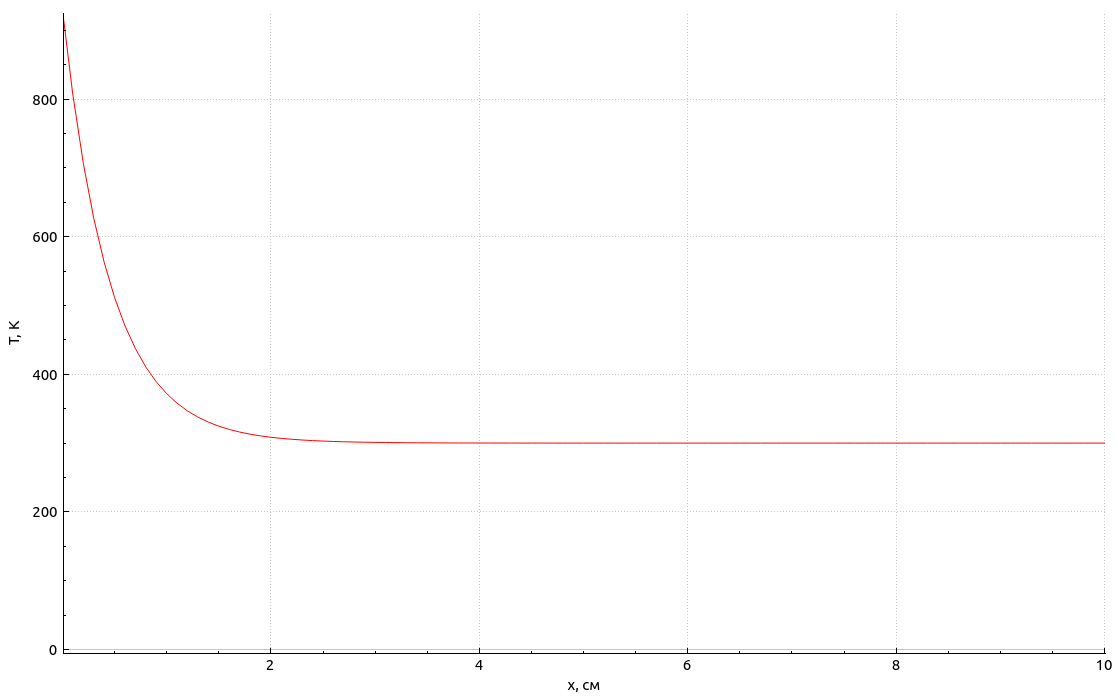
\includegraphics[width=\linewidth]{inc/img/graph1}


	\item \textbf{График зависимости $T(x)$ при $F_0=-10$ Вт/см$^2$}

	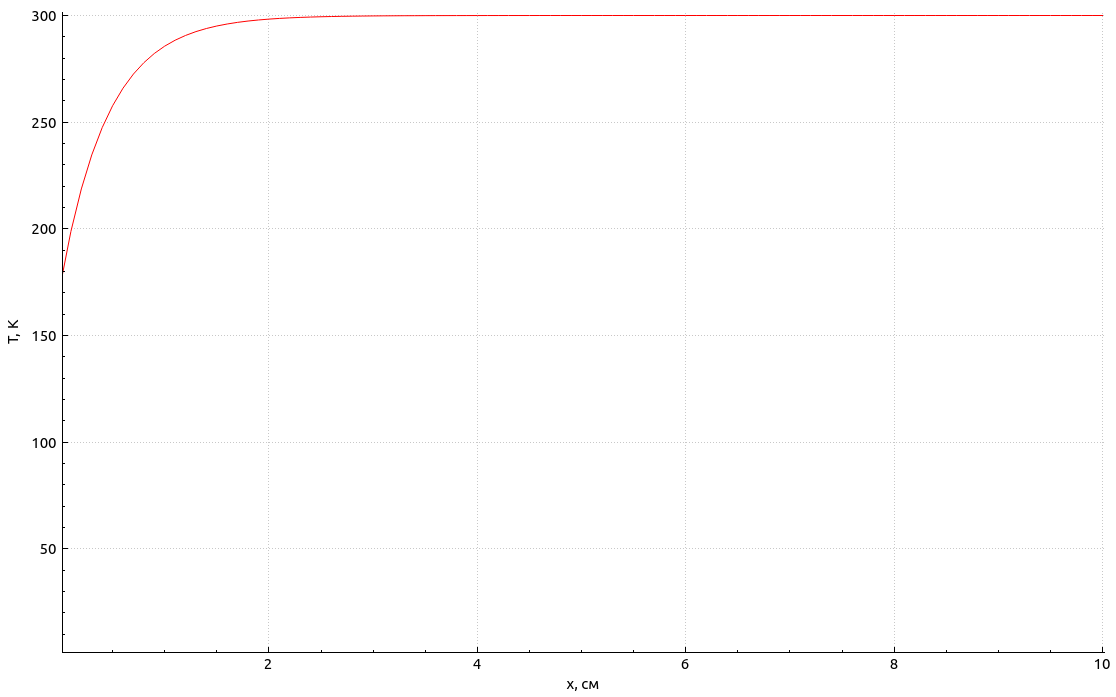
\includegraphics[width=\linewidth]{inc/img/graph2}


	\item \textbf{График зависимости $T(x)$ при увеличенных в 3 раза значениях $\alpha(x)$}

	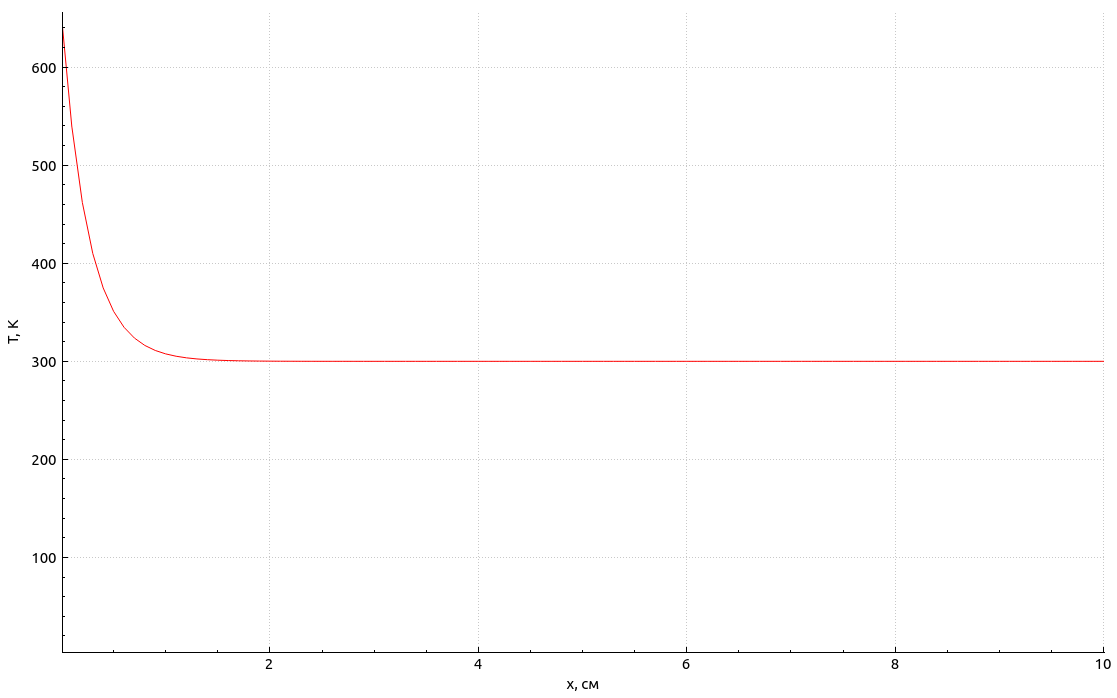
\includegraphics[width=\linewidth]{inc/img/graph3}

	\pagebreak
	\item \textbf{График зависимости $T(x)$ при $F_0=0$}

	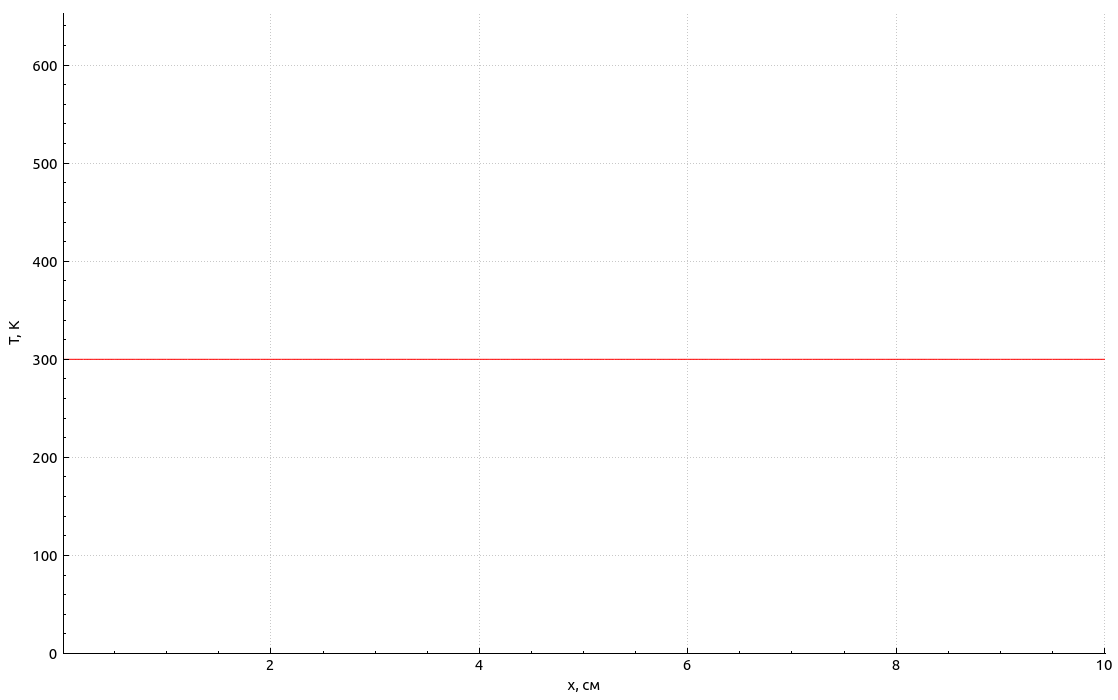
\includegraphics[width=\linewidth]{inc/img/graph4}
\end{enumerate}

\section*{Вопросы}

\begin{enumerate}
	\item \textbf{Какие способы тестирования программы можно предложить?}

	\begin{itemize}
		\item Задать отрицательный тепловой поток.
		Стержень будет охлаждаться с левого торца, а значит $T(x)$ от $0$ до $l$ будет увеличиваться.

		\item При большей теплоотдачи стержня его температура должна снизиться.

		\item При нулевом тепловом потоке температура стержня должна быть неизменной и равняться температуре окружающей среды.
	\end{itemize}

	\item \textbf{Получите простейший разностный аналог нелинейного краевого условия при}
	\begin{equation}
		x=l,\quad-k(x)\frac{\mathrm dT}{\mathrm dx} = \alpha_N\left(T(l)-T_0\right)+\varphi(T).
	\end{equation}

	Аппроксимируем производную односторонней разностью
	\begin{equation}
		-k_l\frac{T_l-T_{l-1}}h=\alpha_N(T_l-T_0)+\varphi(T_l).
	\end{equation}
	Отсюда
	\begin{equation}
		-(k_l+\alpha_Nh)T_l+k_lT_{l-1}=\varphi(T_l)h-\alpha_NhT_0
	\end{equation}


	\item \textbf{Опишите алгоритм применения метода прогонки, если при $x=0$ краевое условие линейное (как в настоящей работе), а при $x=l$, как в п. 2.}

	\begin{equation}
		\left\{
		\begin{aligned}
			x&=0,\quad-k(0)\frac{\mathrm dT}{\mathrm dx}=F0,\\
			x&=l,\quad-k(l)\frac{\mathrm dT}{\mathrm dx}=\alpha_N(T(l)-T_0)+\varphi(T).
		\end{aligned}
		\right.
	\end{equation}

	Будем использовать левую прогонку, основная прогоночная формула:
	\begin{equation}
		y_n = \xi_{n-1} y_{n-1} + \eta_{n-1}
		\label{eqn:12}
	\end{equation}

	Принимая простейшую (первого порядка точности) аппроксимацию краевого условия при $x=0$, получим его разностный аналог:
	\begin{equation}
		-k_0\frac{T_1-T_0}h=F_0 \quad\Rightarrow\quad -k_0T_1+k_0T_0=F_0h.
	\end{equation}
	Сравнивая с \eqref{eqn:12} при $n=1$:
	\begin{equation}
		\left\{
		\begin{aligned}
			\xi_0 &= 1,\\
			\eta_0 &= -\frac{F_0h}{k_0}.
		\end{aligned}
		\right.
	\end{equation}

	Аналогично, разностная аппроксимация правого краевого условия имеет вид:
	\begin{gather}
		-(k_l+\alpha_Nh)T_l+k_lT_{l-1}=\varphi(T_l)h-\alpha_NhT_0,\\
		-(k_l+\alpha_Nh)T_l+k_l\frac{T_l-\eta_{l-1}}{\xi_{l-1}}=\varphi(T_l)h-\alpha_NhT_0.
	\end{gather}

	Отсюда получаем уравнение для определения $T_0$:
	\begin{equation}
		\varphi(T_l)h - \left(k_l+\alpha_Nh-\frac{k_l}{\xi_{l-1}}\right)T_l = \frac{k_l\eta_{l-1}}{\xi_{l-1}}-\alpha_NhT_0.
	\end{equation}


	\item \textbf{Опишите алгоритм определения единственного значения сеточной функции $y_p$ в одной заданной точке $p$.
	Использовать встречную прогонку, т. е. комбинацию правой и левой прогонок} (\href{ftp://eufs.bmstu.ru/19426610-bd1a-11e6-93f1-005056960017/30-03-2020-%D0%9B%D0%B5%D0%BA%D1%86%D0%B8%D1%8F_%E2%84%968_%D0%9C%D0%BE%D0%B4%D0%B5%D0%BB%D0%B8_%D0%9E%D0%94%D0%A3_%D0%BA%D1%80%D0%B0%D0%B5%D0%B2%D0%B0%D1%8F_%D0%B7%D0%B0%D0%B4%D0%B0%D1%87%D0%B0.pdf}{Лекция №8}).
	\textbf{Краевые условия линейные.}

	Пусть $i=p$, где $0<p<N$.
	Тогда в области $0 \leqslant i \leqslant p+1$ прогоночные коэффициенты $\alpha_i, \beta_i$ (правая прогонка):
	\begin{equation}
		\alpha_{i+1}=\frac{C_i}{B_i-\alpha_iA_i},\quad \beta_{i+1}=\frac{A_i\beta_i+D_i}{C_i-\alpha_iA_i}
	\end{equation}
	А в области $p\leqslant i \leqslant N$ прогоночные коэффициенты $\xi_i, \eta_i$ (левая прогонка):
	\begin{equation}
		\xi_{i}=\frac{C_i}{B_i-\xi_{i+1}A_i},\quad \eta_{i}=\frac{A_i\eta_{i+1}+D_i}{B_i-\xi_{i+1}A_i}.
	\end{equation}

	Тогда при $i=p$:
	\begin{equation}
		y_p=\alpha_{p+1}y_{p+1}+\beta_{p+1},~~y_{p+1}=\xi_{p+1}y_{p}+\eta_{p+1},
	\end{equation}
	и тогда:
	\begin{equation}
		y_{p}=\frac{\beta_{p+1}+\alpha_{p+1}\eta_{p+1}}{1-\alpha_{p+1}\xi_{p+1}}.
	\end{equation}
\end{enumerate}

\pagebreak
\section*{Листинг}

\lstinputlisting[caption={\code{solve.hpp}}, language=C++]{../solve.hpp}

\lstinputlisting[caption={\code{solve.cpp}}, language=C++]{../solve.cpp}

\end{document}



\section*{Виртуальная файловая система}



\begin{figure}[H]
	\centering
	\includegraphics[width=\linewidth]{inc/img/myfs}
	\caption{Демонстрация работы программы}
	\label{img:myfs}
\end{figure}

\end{document}
